\documentclass[uplatex,dvipdfmx]{jsarticle}
\usepackage{geometry}
\usepackage{hyperref}
\usepackage{csvsimple}
\usepackage{float}
\usepackage{url}
\usepackage[uplatex,deluxe]{otf} % UTF
\usepackage[noalphabet]{pxchfon} % must be after otf package
\usepackage{graphicx}
\usepackage[fleqn,tbtags]{mathtools} % 数式関連 (w/ amsmath)

\geometry{a4paper, margin=1in}
\begin{document}

\title{BBS 掲示板 仕様書}
\author{24G1001 相京 航汰}
\date{2024年1月7日}
\maketitle

\section{利用者向け}

\subsection*{画面のレイアウト}
- \textbf{掲示板ページ (bbs.html)}
  \begin{itemize}
    \item ページのタイトル: \textbf{掲示板}
    \item ページ構成:
      \begin{itemize}
        \item \textbf{投稿フォーム:}
          \begin{itemize}
            \item 名前を入力するテキストボックス
            \item メッセージを入力するテキストボックス
            \item 投稿ボタン
          \end{itemize}
        \item \textbf{投稿一覧エリア:}
          \begin{itemize}
            \item 投稿内容が表示される.
            \item 各投稿には以下の要素が表示される:
              \begin{itemize}
                \item 名前
                \item メッセージ
                \item いいねボタン
                \item 編集ボタン
                \item 削除ボタン
              \end{itemize}
          \end{itemize}
        \item \textbf{投稿チェックボタン:} 投稿の更新状況を確認するボタン
      \end{itemize}
  \end{itemize}

\subsection*{ボタンの動作}
\begin{enumerate}
  \item \textbf{送信ボタン}
    \begin{itemize}
      \item 名前とメッセージを入力して押すと,その内容が新しい投稿として追加される.
      \item 投稿後は入力欄がクリアされ,投稿一覧が更新される.
    \end{itemize}

  \item \textbf{投稿チェックボタン}
    \begin{itemize}
      \item サーバーに現在の投稿数を問い合わせ,更新があれば新しい投稿を一覧に追加する.
    \end{itemize}

  \item \textbf{いいねボタン}
    \begin{itemize}
      \item ボタンを押すと,その投稿に「いいね」が1つ追加される.
      \item クリック後,ボタンに表示される「いいね数」が更新される.
    \end{itemize}

  \item \textbf{編集ボタン}
    \begin{itemize}
      \item ボタンを押すとポップアップが表示され,メッセージの編集が可能になる.
      \item 編集後,サーバーに変更が送信され,投稿が更新される.
    \end{itemize}

  \item \textbf{削除ボタン}
    \begin{itemize}
      \item ボタンを押すとその投稿が削除される.
      \item 削除後,画面から投稿が消える.
    \end{itemize}
\end{enumerate}


\section{管理者向け}

\subsection*{サーバーの起動手順}
\begin{enumerate}
  \item \textbf{前提条件}
    \begin{itemize}
      \item Node.js および npm がインストールされていること.
      \item 必要なモジュールがインストールされていること.
     \end{itemize}

  \item \textbf{サーバーの起動}
    \begin{verbatim}
    node app8.js
    \end{verbatim}
    \begin{itemize}
      \item サーバーはデフォルトでポート \texttt{8080} で動作する.
    \end{itemize}

  \item \textbf{サーバーの停止}
    \begin{itemize}
      \item サーバーを停止するには、起動中のターミナルで \texttt{Ctrl + C} を押す.
    \end{itemize}

  \item \textbf{ブラウザでの確認}
    \begin{verbatim}
    http://localhost:8080/public/bbs.html
    \end{verbatim}
\end{enumerate}

\subsection*{ファイル構成}
\begin{itemize}
  \item \textbf{app8.js:} サーバーサイドのコード.
  \item \textbf{bbs.html:} クライアントのHTML.
  \item \textbf{bbs.js:} クライアントのJavaScript.
  \item \textbf{bbs.css:} クライアントのスタイルシート.
\end{itemize}

\newpage

\section{開発者向け}

\begin{figure}[H]
   \centering
   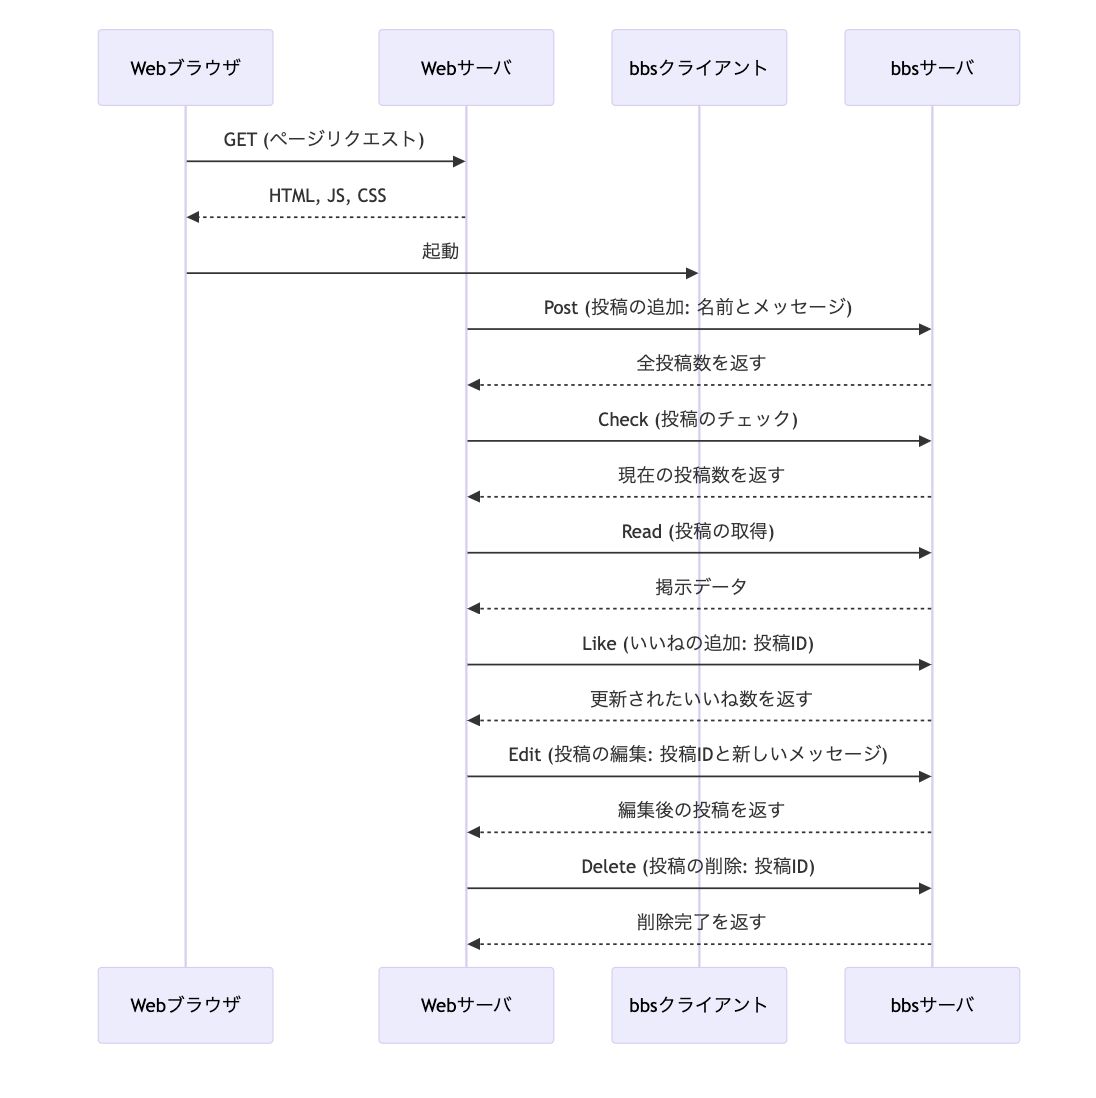
\includegraphics[width=15cm]{nagare.png}
   \caption{掲示板システムの全体の流れ}
   \label{nagare}
\end{figure}


\subsection*{プログラム概要}

\subsubsection*{サーバーサイド (app8.js)}
- \textbf{フレームワーク:} 
- \textbf{主なエンドポイント:}
  \begin{tabular}{|l|l|l|}
  \hline
  HTTPメソッド & URL        & 説明 \\
  \hline
  POST         & /post      & 新しい投稿を追加する \\
  POST         & /check     & 投稿数を確認する \\
  POST         & /read      & 新しい投稿を取得する \\
  POST         & /like      & 投稿にいいねを追加する \\
  POST         & /edit      & 投稿を編集する \\
  POST         & /delete    & 投稿を削除する \\
  \hline
  \end{tabular}

- \textbf{データ形式:}
  \begin{itemize}
    \item リクエストは \texttt{application/x-www-form-urlencoded} 形式.
    \item レスポンスは JSON 形式.
  \end{itemize}
  
\subsection*{application/x-www-form-urlencoded形式とは}
application/x-www-form-urlencoded は,Webフォームから送信されるデータのエンコーディング形式の一つである.この形式は,HTTP リクエストのボディ部分でデータを送信する際に使用され,特に GET または POST メソッドでよく利用される.例えば,ウェブフォームを使ってユーザーが入力した情報をサーバーに送信する際に,この形式でデータが送られる.採用理由は,簡単で広くサポートされているからであり,この形式は,HTTPリクエストの標準的なデータ形式として広く認識されており,ほとんどのサーバーおよびクライアントライブラリでサポートされている.Webフォーム(例えば,HTMLフォーム)から送信されるデータは,この形式でエンコードされるのが一般的である.

\subsubsection*{主な関数}
\begin{itemize}
  \item \textbf{投稿の追加 (/post)}
    \begin{itemize}
      \item リクエストボディ例:
        \begin{verbatim}
        name=ユーザー名&message=投稿内容
        \end{verbatim}
      \item レスポンス例:
        \begin{verbatim}
        { "number": 3 }
        \end{verbatim}
    \end{itemize}

  \item \textbf{投稿のチェック (/check)}
    \begin{itemize}
      \item リクエストボディ: 空
      \item レスポンス例:
        \begin{verbatim}
        { "number": 3 }
        \end{verbatim}
    \end{itemize}

  \item \textbf{投稿の取得 (/read)}
    \begin{itemize}
      \item リクエストボディ例:
        \begin{verbatim}
        start=0
        \end{verbatim}
      \item レスポンス例:
        \begin{verbatim}
        {
          "messages": [
            { "id": 1, "name": "Alice", "message": "Hello!", "likes": 2 },
            { "id": 2, "name": "Bob", "message": "Hi there!", "likes": 1 }
          ]
        }
        \end{verbatim}
    \end{itemize}

  \item \textbf{いいねの追加 (/like)}
    \begin{itemize}
      \item リクエストボディ例:
        \begin{verbatim}
        id=1
        \end{verbatim}
      \item レスポンス例:
        \begin{verbatim}
        { "likes": 3 }
        \end{verbatim}
    \end{itemize}

  \item \textbf{投稿の編集 (/edit)}
    \begin{itemize}
      \item リクエストボディ例:
        \begin{verbatim}
        id=1&message=新しいメッセージ
        \end{verbatim}
      \item レスポンス例:
        \begin{verbatim}
        {
          "updatedPost": { "id": 1, "name": "Alice", "message": "新しいメッセージ", "likes": 2 }
        }
        \end{verbatim}
    \end{itemize}

  \item \textbf{投稿の削除 (/delete)}
    \begin{itemize}
      \item リクエストボディ例:
        \begin{verbatim}
        id=1
        \end{verbatim}
      \item レスポンス例:
        \begin{verbatim}
        { "message": "Post deleted" }
        \end{verbatim}
    \end{itemize}
\end{itemize}

\subsubsection*{クライアントサイド}
- \textbf{bbs.js:}
  \begin{itemize}
    \item 各ボタンに対応するイベントリスナーを定義.
    \item サーバーと通信し,投稿データを更新・取得.
  \end{itemize}

- \textbf{bbs.css:}
  \begin{itemize}
    \item 投稿エリアのレイアウトをスタイル定義.
  \end{itemize}

\section{ソースコード}
\url{https://github.com/Kooxxx/webpro_06.git}

\end{document}
